
\documentclass{sig-alternate}

\usepackage{graphicx}
\usepackage{url}
\usepackage{listings}
\usepackage{color}
\hyphenation{Block-Py}
\newcommand\TODO[1]{{[\color{red}#1]}}

\newcommand{\compresslist}{%
\setlength{\itemsep}{1pt}%
\setlength{\parskip}{0pt}%
\setlength{\parsep}{0pt}%
}

\begin{document}

\title{Implementing an Open-access, Data-Science Programming Environment for Everyone}
\numberofauthors{1}
\author{
	\alignauthor{Removed}\\
	\email{Removed}\\
	\affaddr{Removed} \\
	\affaddr{Removed}  \\
%  	\alignauthor {Austin Cory Bart, Eli Tilevich, Clifford A. Shaffer, and Dennis G. Kafura}\\
%	\email{\{acbart, tilevich, shaffer, kafura\}@vt.edu}\\
%\affaddr{Computer Science} \\
%	\affaddr{Virginia Tech}  \\
}

\maketitle
\begin{abstract}
 Learners new to computing face the challenge of mastering programming fundamentals while remaining sufficiently motivated to engage with the computing discipline.
In particular, students outside of Computer Science majors can struggle to find relevance in traditional computing curricula that tend to either emphasize abstract concepts, focus on non-practical entertainment (e.g., game and animation design), or rely on decontextualized settings.
To address these issues, this paper introduces BlockPy, a block-based environment for Python (http://blockpy.com). BlockPy is a web-based, open-access programming environment that supports introductory programming with an emphasis on data science.
By supporting the latest LTI standards, it can work for informal learners and formal class settings.
BlockPy can be configured to provide guiding feedback for its interactive programming problems in order to support learners at their own pace.
It promotes long-term transfer by scaffolding an introduction to textual programming (Python) through a block-based programming view that is ideal for beginners of any background.
We present the results from a pilot study of BlockPy's use.
\end{abstract}

% A category with the (minimum) three required fields
\category{K.3.2}{Computer and Information Science Education}{Computer Science Education}

\terms{Design, Human Factors, Reliability, Experimentation}

\keywords{Blockly, Blockpy, Python, Data Science, Guided Practice}

\section{Introduction}

A growing population of non-CS majors are entering introductory computing courses, under the banner of subjects such as Computational Thinking.
These students have little experience with programming and computing, low self-efficacy, and are uncertain about the value of computing towards their long-term career goals.
Some of these students voluntarily enroll in computing courses, but others are being forced to as part of new university requirements.
Echoing a popular sentiment among CS educators, 
\textit{``At the novice programming level, blocks-based languages are the most promising direction today''}~\cite{guzdial-blocks}.
Our solution to serve this population is BlockPy: a web-based, dual-text/block Python environment for data science (\url{http://think.cs.vt.edu/blockpy/}).

\textbf{Why Data Science?}
Modern approaches to contextualizing introductory courses have focused on making the experience ``fun'' and ``interesting'', with an emphasis on game design and media computation~\cite{systematic-review}.
However, student motivation is a complex, multi-faceted construct dependent on more than just situational interest; in particular, holistic models of motivation suggest that students also need to feel that long-term career goals are being satisfied~\cite{jones-description}.
Despite an attempt at convincing students otherwise, Media Computation is not perceived as an authentically useful context for non-majors, based ona  study by Guzdial et al~\cite{guzdial2006imagineering}.

We suggest that Data Science is a more motivating context, thanks to the wide-spread need for data processing in other majors.
Students are often enrolling in computing courses to learn how to manage the dizzying quantities of data being stored, used, and analyzed in their discipline.
By grounding classwork in this context, students can be more easily convinced of the relevance of computing.
By aligning the context with students' long-term needs, students can also learn skills more relevant to their needs.
Finally, data science as a context naturally lends itself to teaching topics related to structured data, iteration, and other core material, making it a pedagogically valuable context to the CS instructor.

\textbf{Why Python?}
Python has become one of the most popular introductory programming languages~\cite{guo2014python}, thanks to its simple syntax but impressive power, including strong support for data science thanks to popular libraries like MatPlotLib.
Its wide-spread use in introductory classes, especially for non-majors, led to our choice.

\textbf{Why Blocks?}
However, any kind of programming is still a challenge to beginners, due to the nature of coding as the ``most powerful, but least usable human-computer interface ever invented.''~\cite{koh-ui-programming}
Block-based languages have been shown to mitigate the start-up time for students to start programming and accomplishing tasks~\cite{bbl-Price, WeintropIcer}.
By providing structure and an immediate view into the entire user interface of a language, blocks greatly benefit introductory learners.

\begin{figure*}[ht]
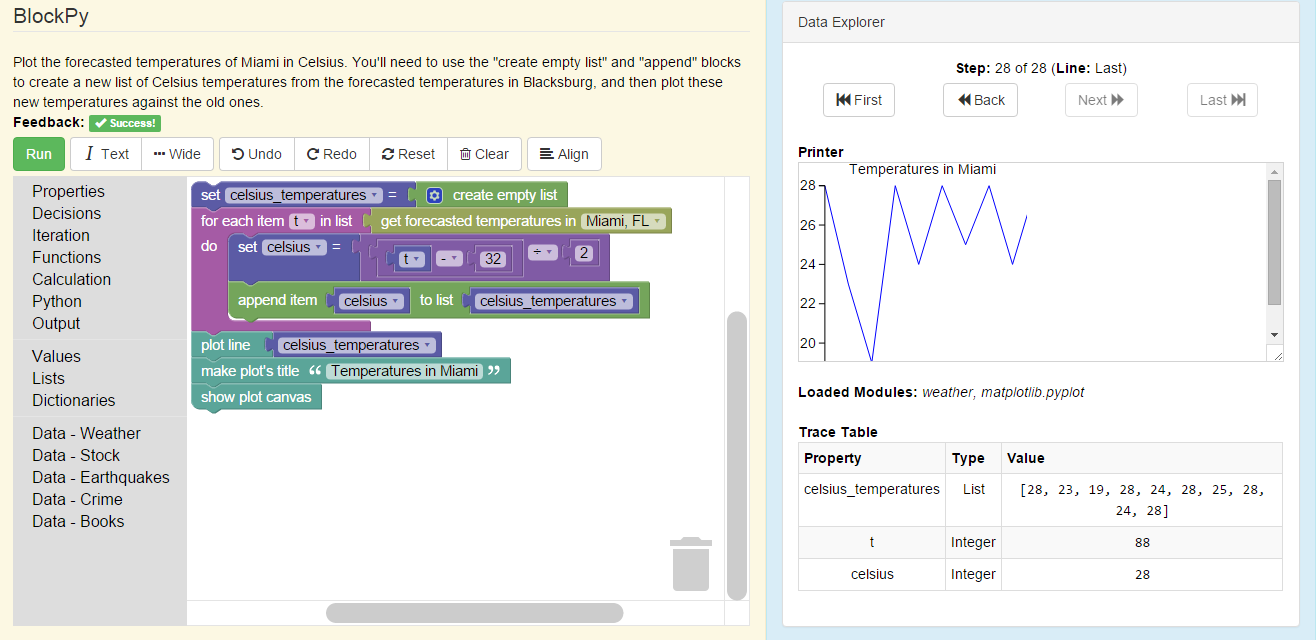
\includegraphics[width=\textwidth]{images/blockpyExample}
\label{fig-blockpy-full}
\caption{A complete screenshot of BlockPy in action}
\end{figure*}

\textbf{Why Another Python Web Environment?}
There are several environments available today that let students and instructors write Python in the browser, including CodeSkulptor~\cite{CodeSkulptor-Tang}, Pythy~\cite{pythy}, and the Online Python Tutor~\cite{Guo:2013}.
BlockPy stands on the shoulders of giants, integrating features inspired by these environments and introducing novel ones.
But none of these existing Python environments scaffolds transitioning students into textual programming languages.

BlockPy was designed to provide dual support for both block-based and text-based code authoring.
At any time, the student can switch freely between a block-based view of their code and a traditional text-based view.
This powerful feature is inspired by Pencil Code, which uses its own Logo language~\cite{Bau}, and similar implementations have been successful as a fading scaffold for students~\cite{Matsuzawa}.

BlockPy extends Pythy's~\cite{pythy} support for ``assignments'', which are problems that integrate presentation with assessment.
However, Pythy only supports traditional unit testing to provide students with feedback, while BlockPy provides an API for code analysis and free-form text guidance that instructors can configure to give helpful suggestions to their students.
Furthermore, Pythy has limited support for data science, whereas BlockPy has a rich library of data sources to draw on and a MatPlotLib-based plotting API.

CodeSkulptor, Pythy, and BlockPy all use the same internal engine for running Python code (``Skulpt''). 
Although CodeSkulptor has an extensive API for creating user interfaces and games, it suffers from using a non-standard library.
Although suitable for beginners, this library does not aid the transition to textual programming languages.
In BlockPy, the philosophy is to maintain compatibility with existing systems when possible.
Instead of a custom plotting API, for instance, we mimic the MatPlotLib interface.

Finally, OnlinePythonTutor has proven to be an incredibly useful tool for visualizing program state in Python programs.
However, we hypothesize that the depth of detail that it gives can be overwhelming for introductory students (e.g., the visualizations use terminology such as Frames and Objects, which might be foreign to students despite being proper terminology).
BlockPy's state explorer does not attempt to match Python Tutor's thoroughness or accuracy, but instead is targeted at providing as helpful as picture of program state as possible within the constraint of simplicity.
This includes highlighting data types and console output as part of the visualizers' program  state, as shown in Figure ~\ref{fig-blockpy-full} on the right side.
Additionally, we remove PythonTutor's server-based python dependency by relying on Skulpt, which works entirely in the students' browser.

\section{BlockPy}

The primary goals of BlockPy are as follows.
\vspace{-\medskipamount}

\begin{enumerate}\compresslist
\item Promote authenticity by empowering students to complete real-world problems.
\item Promote maturity by faded scaffolds (e.g., transitioning from blocks to text).
\item Minimize the need for help from instructors and teaching assistants.
\end{enumerate}

\subsection{Python Execution}

Python Code Execution is achieved through a modified instance of the Skulpt JavaScript library.
Skulpt is a full Python parser and compiler, supporting almost all of the language features and generating runnable JavaScript code.
The Skulpt execution environment resides entirely within the users' browser, so there is no reliance on an external server.
The long-term goal of this project is to support a set of rich libraries so that sophisticated applications can be developed --- beyond console-based problems.

\subsection{Data Science Blocks}

BlockPy focuses on Data Science as its primary context, and so we have specific blocks and APIs for working with data.
We use an existing fork of Skulpt with the popular MatPlotlib library, and extended it with our own implementation of the CORGIS project~\cite{CORGIS}.
The MatPlotLib API, for example, provides a ``plot(list)'' function to create simple line plots.
By basing everything around MatPlotLib, students can seamlessly shift to a serious Python programming environment without loss of code or productivity. 

The CORGIS (Collection of Real-time, Giant, Interesting, dataSets) Project seeks to make motivating datasets available to introductory students through simple programming libraries~\cite{CORGIS}.
For instance, up-to-date temperature and humidity reports for American cities are available through the Weather library, 
These datasets are drawn from many disciplines, resulting in material meant to be universally interesting and relevant.
These datasets are also equipped with scaffolding that simplifies the process of working with what are sometimes complicated data sources.

\begin{figure}
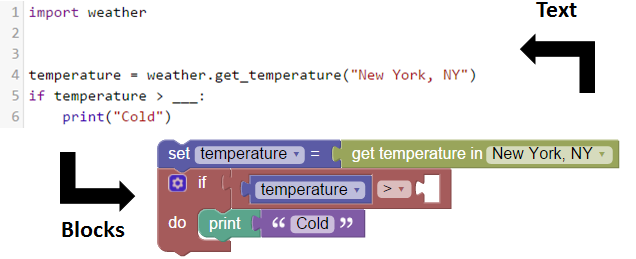
\includegraphics[width=0.5\textwidth]{images/mltExample}
\label{fig-mlt-user}
\caption{User perspective of block/text transition}
\end{figure}

\begin{figure}
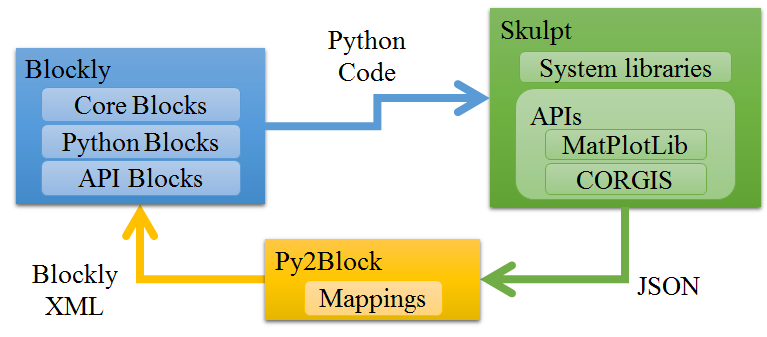
\includegraphics[width=0.5\textwidth]{images/mltOverview}
\label{fig-mlt-architecture}
\caption{Architectural perspective of the block/text transition}
\end{figure}

\subsection{Mutual Language Translation}

One of the largest technical contributions of this project is the Mutual Language Translation between Blockly and Python.
Figure \ref{fig-mlt-architecture} gives an overview of the technical architecture used to achieve this translation.
Blockly outputs valid python source code, which can be passed into Skulpt in order to extract a JSON representation of the Abstract Syntax Tree.
Alternatively, the Python source of the Skulpt program can be edited directly in the Text view. 
Either way, this AST is parsed using our Py2Block library to generate an XML representation that Blockly can render in the Block View.
Figure \ref{fig-mlt-user} demonstrates the users' experience.

Blockly already supports compilation of its blocks to Python, JavaScript, PHP, and Dart.
However, this multiple language support comes at a cost of reduced isomorphism---each language has different syntax for their common operations, and it is impossible to create a fully-featured block language with a one-to-one mapping between them.
For example, JavaScript has no support for parallel assignment, a commonly-used feature in Python, while Python does not have a unary increment operator.
Blockly itself has syntax and vocabulary descended from Logo.

Instead of trying to satisfy multiple languages, we have dropped support for JavaScript and the rest in favor of a more full-featured mapping to Python.
This requires minor changes that introduce Python-centric syntax details:
function blocks are labeled ``define'', assignment blocks have an ``='' symbol, the ``add item to list'' block is renamed to ``append''.
Blockly has also been extended with new language features, including dictionary access and creation.

Eventually, the interface should offer a complete isomorphic mapping to Python.
However, there are a number of complications to resolve before that can occur.
For instance, Python uses square brackets for both list indexing and dictionary access.
There is a strong desire to differentiate between these types of access, visible in the block view as two distinct kinds of blocks (``get ith element of list'' vs. ``get key from dict'' blocks).
However, depending on what features of python are supported, it can be difficult or even impossible to statically identify the usage of a given pair of brackets-- sophisticated program analysis techniques are needed.

A less technical and more user-oriented question is how many language details should be exposed, and at what rate.
A rarely used feature of ``for'' loops in Python is to contain an ``else'' clause that is executed upon successful completion of the loop (that is, when it is not prematurely escaped using a ``break'' statement).
This advanced language feature is meant to draw special attention to connected actions that must be performed after the iteration is completed (similar to a ``finally`` statement).
If an ``else'' clause were made available to beginners first trying to grapple with iteration, it is likely they would confuse the concept with the conditional ``else'' clause used in ``if'' statements.
Cognitive Load Theory can be a harsh mistress for beginners, and the user interface needs to avoid exposing unnecessary details where possible.
While this is a clear case, there more subtle examples.
It can be very difficult to recognize when the learner is ready to use parallel assignment, and therefore able to specify multiple variables on the left side of an assignment block.
A block-based language forces a teacher to make important decisions about how to expose language features.

\subsection{Parson's Problems}

Parsons' Problems are a special type of coding exercise where all of the necessary code blocks are present, but disconnected and shuffled.
BlockPy supports these types of problems with a special ``Parsons Mode'' where top-level blocks are constantly shuffled in the block-mode.
When a student tries to convert code with disconnected blocks, the generated Python code will be filled in with triple underscores, as demonstrated in Figure~\ref{fig-mlt-user}.
These underscores (usually valid syntax in Python) will trigger a runtime error, encouraging students to think critically about their code.

\begin{figure}
\begin{center}
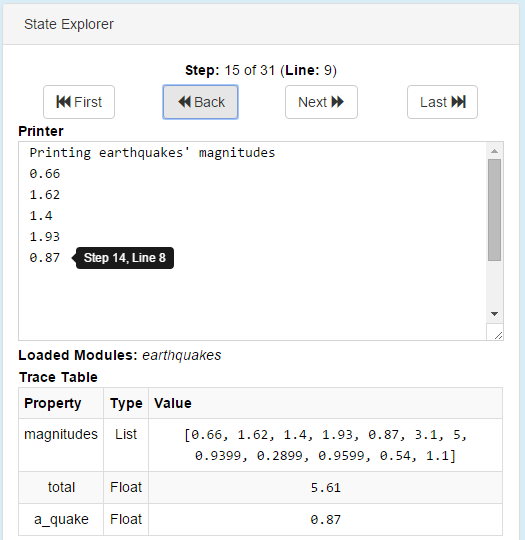
\includegraphics[width=0.4\textwidth]{images/blockpyStateExplorer}
\end{center}
\label{fig-state-explorer}
\caption{The State Explorer displays information about the entire state of the program, including output and loaded modules.}
\end{figure}

\subsection{State Explorer}

A common debugging tool in many modern IDEs is a Variable Explorer, used to trace the programs' execution over time.
BlockPy expands this concept into a State Explorer. 
The State Explorer displays more than just information about variables - the dashboard also reveals information about what has been printed 
Users can step through the code's execution, affecting what is currently printed, imported, and the values of the variables.
The relevant blocks or text are also highlighted.

\begin{figure}
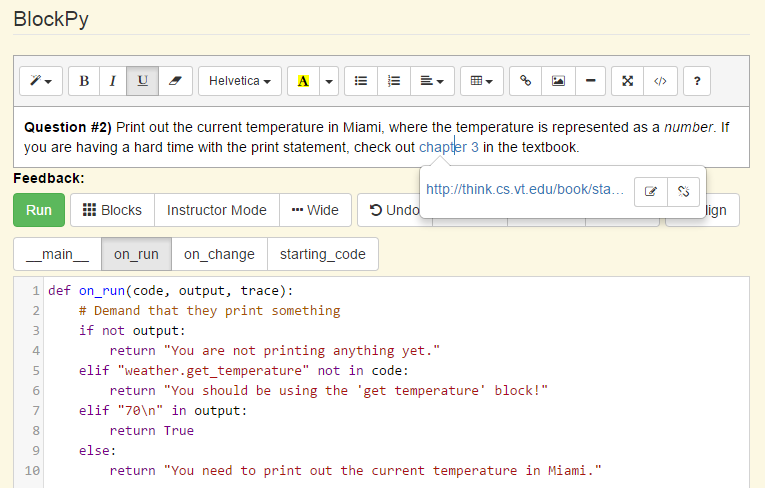
\includegraphics[width=0.5\textwidth]{images/blockpyTeacherEditing}
\label{fig-teacher-view}
\caption{Instructor Mode lets you edit questions and and define special functions to give feedback.}
\end{figure}

\subsection{Guided Practice}

A limitation of programming environments like Snap! is that they are not pedagogically interactive --
students completing an assignment in the system are not guided to success.
One of the most powerful features of BlockPy is the interactive feedback feature.
When students run their code, it is checked against instructor-provided logic.
If the student code fails for some reason, they are offered a suggestion or motivational remark.
Correct code gives a green checkmark.

In the Instructor Mode (shown in Figure~\ref{fig-teacher-view}), instructors can provide a problem description using a rich text editor and edit an ``on\_run'' function (using the regular text/block interface that students use).
This ``on\_run'' function is the interface for providing feedback, consuming the students code, their final output, and a complete trace of their programs state.
The complete API is evolving based on common use cases, such as checking whether a student is iterating over a non-empty list (a surprisingly common problem).

\subsection{LTI Support}

A growing cause for alarm in the education community is the ever-expanding array of third-party tools that demand control over students data.
The BlockPy project is committed to supporting LTI technology to reduce instructors dependency on BlockPy for course management.
LTI (Learning Technology Interoperability) is a mechanism by which instructors can embed questions in their existing course management software (e.g., Canvas, OpenEdX) and receive assignment outcomes such as performance and participation data.
As LTI version 2.0 rolls out in the coming year, we are working to support the latest standard.

\subsection{Missing features}

Mutual Language Translation is being developed on a per-feature basis.
Unfortunately, this means that a number of advanced Python features are currently not supported.
Perhaps the biggest omission is the lack of support for Classes.
A number of other features are omitted too, at the time of writing: tuples, list comprehensions, and while loops, for example.
This does not mean that students cannot write programs featuring classes or these features.
Python code using these features will render in BlockPy as embedded text blocks, rather than as regular blocks.
There is no technical impediment to supporting these features, the process is limited only by time and community interest.

\section{Pilot Study}

BlockPy has been piloted in an introductory ``Computational Thinking'' course with 35 students.
These students come from a diverse range of majors, including liberal arts (57\%), architecture (17\%),  sciences (15\%), and others (11\%).
There were 20 female students (57\%) and 15 male.
The vast majority of students reported no prior experience with programming or Computer Science, with less than 17\% having taken the high school AP course.
They were evenly distributed across years, with slightly more senior (29\%), equal percentages of sophomore and juniors (26\%), and fewer freshmen (14\%).
Although small, the student demographics reflect our ideal population. 

The Computational Thinking course's content is focused on teaching Abstraction and Algorithms.
While programming is not a primary learning objective, it is an important topic in the course as a tool of concretely talking about the higher level objectives.
The first third of the course, students work with NetLogo (although they do not program in it, they only read code) and participate in a number of explanatory kinesthetic activities.
Then they are introduced to Python using BlockPy, for which they spend roughly six classes on completing guided practice problems in a mastery style (that is, they are allowed an infinite number of retries).
The next two classes are devoted to using a regular Python environment (Spyder) to complete small programming assignments (similar to the ones done with BlockPy).
Finally, students are given eight class periods to work on their individual final project in Spyder.

\subsection{Methodology}

Every student interaction was logged by the system, including changes to the students' code.
This data was also correlated to two surveys, one given after the BlockPy section and the other given at the end of the course.
The survey was composed of Likert questions on a 4-point scale and open-ended qualitative questions.
This gives us a wealth of data to analyze, although the small population size makes it difficult to derive significant results.

\subsection{Perceptions of BlockPy}

\begin{figure}
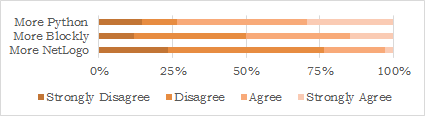
\includegraphics[width=0.5\textwidth]{images/surveyMore}
\label{fig-want-more}
\caption{Do students want more time with NetLogo, BlockPy (Blockly), or Spyder (Python).}
\end{figure}

The first survey question students were asked was about whether they wanted more time with each of the programming environments they used in the course: NetLogo, BlockPy, or Spyder.
The results of this question are shown in Figure~\ref{fig-want-more}.
Note that BlockPy was referred to as ``Blockly'', and the use of the Spyder environment was referred to as ``Python''.
These results suggest that students valued their experiences with BlockPy more than they did with NetLogo, but mostly felt that they were not getting enough Python experience. 
This is backed up by the qualitative data, where some students say ``More Blockly, Less Python'', but others ask for ``More Blockly and More Python''.

\subsection{Usage of BlockPy}

Over the six days spent using BlockPy, students were tasked with 40 classwork questions and 19 homework questions.
Students ran their code an average of four times per problem (standard deviation is ~1.8 times).

Students were asked if they felt successful in the transition from BlockPy to Spyder.
65\% of the class agreed or strongly agreed, suggesting that there was still a sizeable population that still felt uncomfortable during that transition.
The original design of the Mutual Language Translation featured the block and text view simultaneously, side-by-side.
However, analysis of the logs reveals that most students did not take advantage of the feature.
Only 5 students (roughly 15\%) had used the conversion functionality at all, and fewer used it consistently.
It is possible that students were observing the code as it changed, but they were not writing textual code.
It is difficult to say why exactly students did not take advantage of it, and the qualitative data are not helpful.
Our current hypothesis is that students were confused by the interface, which required manual conversion to go from text to blocks.
In our new version, the conversion happens automatically, simply by switching tabs, and we will provide intentional opportunities for the students to switch.

\begin{figure}
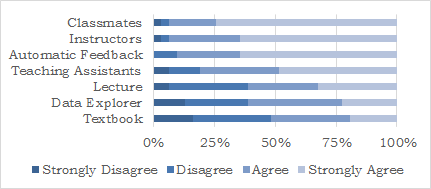
\includegraphics[width=0.5\textwidth]{images/surveyHelpfulness}
\label{fig-survey-helpfulness}
\caption{How helpful to students' learning were these resources?}
\end{figure}

Students were surveyed about what helped their learning the most, and the results are shown in Figure~\ref{fig-survey-helpfulness}.
Peer learning and the instructors were about on par with the automatic feedback given in BlockPy, suggesting the strong value in using such a system.
Despite the popular response to the Data Explorer, relatively few students took advantage of it (11 students, roughly 31\%).
Since more than 50\% of the class reported finding value in the data explorer, it is possible that the students benefited from instructor presentations of the tool, even if they didn't take advantage of it themselves. 

Students did not take advantage of many of BlockPy's most powerful features, suggesting that either further work was required on their interface or students need to be taught how to take advantage of them better.

\begin{figure}
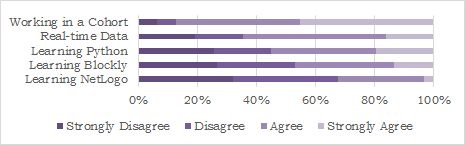
\includegraphics[width=0.5\textwidth]{images/surveyUsefulness}
\label{fig-survey-usefulness}
\caption{How useful to students' long-term career goals was each of the following experiences?}
\end{figure}

\begin{figure}
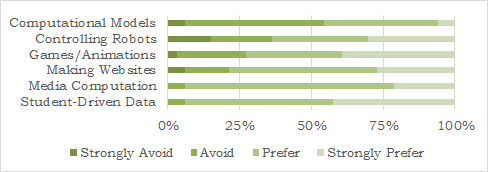
\includegraphics[width=0.5\textwidth]{images/surveyContexts}
\label{fig-survey-context}
\caption{Students preference for different potential introductory contexts.}
\end{figure}

\subsection{Data Science Context}

Students were surveyed about their perceptions of the value of different course experiences with regards to their long-term career goals (Figure~\ref{fig-survey-usefulness}) and their interest in potential contexts for an introductory computing course (Figure~\ref{fig-survey-context}).
Both surveys suggest that students find data science to be compelling, but should be taken with a grain of salt, since students have negligible experience with alternative contexts, despite the care taken in wording the question.
However, our preliminary results are exciting since they suggest that this is an approach worth exploring further.

\subsection{Future Work}

BlockPy represents an ongoing research project and evolving practioners' tool.
We have a number of features planned to expand the support for Python, in particular more blocks for data science explorations.
We are also planning on expanding support for the guided feedback API for instructors and the support available through the compiler, such as leveraging static/dynamic type inference techniques to improve block rendering and error reporting.

We also have a number of research questions posed by the block-based nature of the interface.
One of the biggest values of a block-based environment is that it can immediately expose the breadth of a rich API.
This greatly reduces students' dependency on documentation.
Of course, exposing this breadth can also be a downside, as students might be overwhelmed by the number of features in the interface.
It is an open research question to decide what language features to expose and what rate to expose them at.

One of the major advantages of game and animation design as an introductory context is that they can make abstract concepts concrete. 
Further analysis is needed to determine the trade-offs of using different contexts.
BlockPy can support this by supporting these alternative contexts, such as turtle graphics and media computation libraries.

Despite the substantial data collected in our pilot study, it is difficult to derive conclusive results due to the small population size and the evolving nature of BlockPy.
This academic year, we are conducting follow-up studies on the logged students' code, even as we collect more data on the newest iteration.
We are hopeful that BlockPy will increase its user base, providing a larger sample of learners to conduct research on, and provide more meaningful data.

\section{Conclusion}
In this paper, we have introduced our block-based environment for Python, named BlockPy.
It is open source and available for use at \url{http://think.cs.vt.edu/blockpy/}.
We believe that BlockPy represents a new paradigm for introductory students, blending interactive support with a strong path to programming maturity.
By teaching in the context of data science, we can provide authenticity even as we move students out of the system towards a more serious environment. 
Research with this environment will help answer crucial questions about the value of data science and blocks.


\bibliographystyle{abbrv}
\bibliography{references} 

\end{document}
